\section{Background and The Algorithm}
\label{section:algorithm}
An ideal softmax operator is a parameterized set of operators that:
\begin{itemize}
\item has parameter settings that allow it to approximate maximization arbitrarily accurately to perform reward-seeking behavior;
\item is a non-expansion for all parameter settings ensuring convergence to a unique fixed point;
\item is differentiable to make it possible to improve via gradient-based optimization; and
\item avoids the starvation of non-maximizing actions.
\item Let $X = x_{1},...,x_{n}$ be a vector of values. We define the following operators:
\end{itemize}

% \textbf{Lemma 2}
\begin{figure}[H] %H为当前位置,!htb为忽略美学标准,htbp为浮动图形
\centering %图片居中
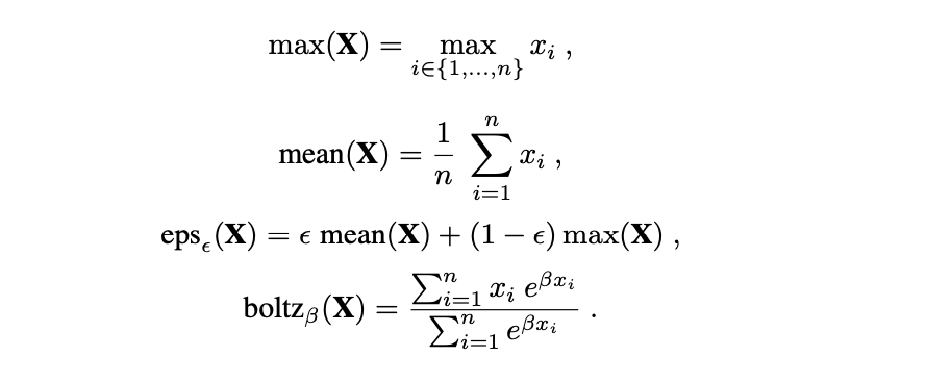
\includegraphics[width=0.7\textwidth]{algorithm.eps} %插入图片,[]中设置图片大小,{}中是图片文件名
% \caption{A list of not ideal softmax operator} %最终文档中希望显示的图片标题
% \label{Fig.main2} %用于文内引用的标签

\end{figure}
The Boltzmann operator $boltz_{\beta}(X)$ is differentiable. It also approximates max as $\beta $→ $\infty$and mean as $\beta $→ $0$ . However, it is not a non-expansion operator, and therefore, the lack of the non-expansion property leads to multiple fixed points and ultimately a misbehavior in learning and planning.
\newpage
\textbf{MellowMax}
\newline\newline
Author presents a new softmax operator that is similar to the Boltzmann operator yet is a non-expansion operator. Author also proves several critical properties of this new operator, introduce a new softmax policy, and present empirical results. The alternative mellowmax softmax operator is defined as follows:
\begin{figure}[H] %H为当前位置,!htb为忽略美学标准,htbp为浮动图形
\centering %图片居中
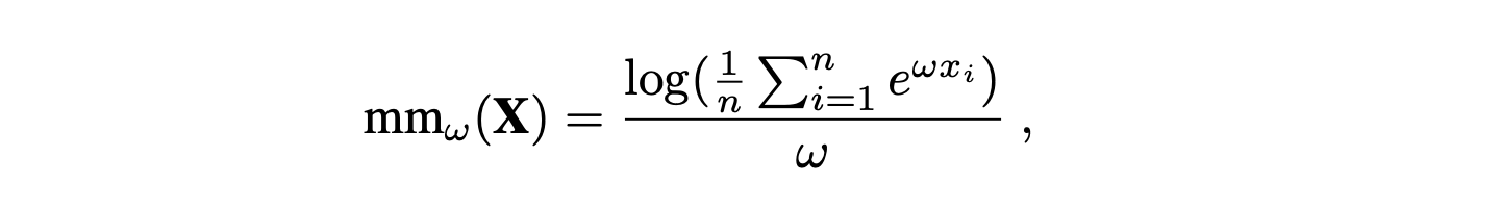
\includegraphics[width=0.7\textwidth]{mel.eps} %插入图片,[]中设置图片大小,{}中是图片文件名
% \caption{mellowmax softmax operator} %最终文档中希望显示的图片标题
% \label{Fig.main2} %用于文内引用的标签

\end{figure}

Author proves that $mm\omega$ is a non-expansion operator, and therefore, GVI and SARSA under $mm\omega$ are guaranteed to converge to a unique fixed point.
Furthermore, the operator acts more and more like pure maximization as the value of $\omega$ is increased. Conversely, as $\omega$ goes to $-\infty$, the operator approaches the minimum.
And as ${\omega}$ gets closer to zero, $mm_{\omega}(x)$ approaches the
mean of the values in $X$.


\textbf{Mellowmax Policy}
\newline\newline
Author formally defines the maximum entropy mellowmax policy of a state $s$ as:
\begin{figure}[H] %H为当前位置,!htb为忽略美学标准,htbp为浮动图形
\centering %图片居中
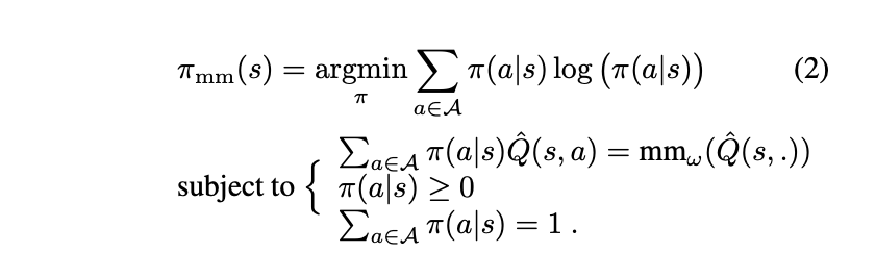
\includegraphics[width=0.7\textwidth]{entropy.eps} %插入图片,[]中设置图片大小,{}中是图片文件名
% \caption{mellowmax softmax operator} %最终文档中希望显示的图片标题
% \label{Fig.main2} %用于文内引用的标签
\end{figure}

After using the method of Lagrange multipliers to solve this system of equations, the probability of taking an action under the maximum entropy mellowmax policy has the form:
\begin{figure}[H] %H为当前位置,!htb为忽略美学标准,htbp为浮动图形
\centering %图片居中
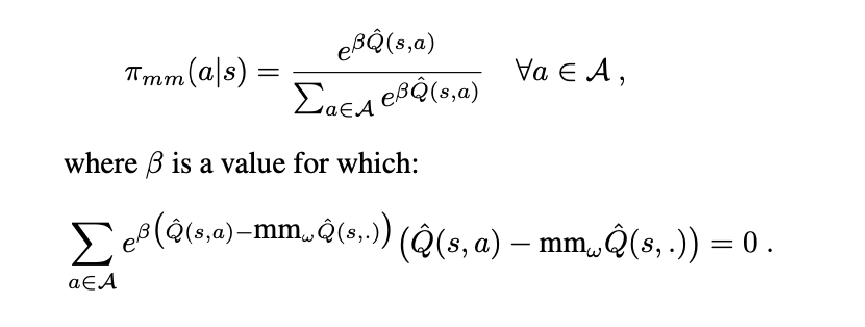
\includegraphics[width=0.7\textwidth]{result.eps} %插入图片,[]中设置图片大小,{}中是图片文件名
% \caption{mellowmax softmax operator} %最终文档中希望显示的图片标题
% \label{Fig.main2} %用于文内引用的标签
\end{figure}

The argument for the existence of a unique root is simple. As $\beta$ → $\infty$, the term corresponding to the best action dominates, and so, the function is positive. Conversely, as $\beta$ → $-\infty$, the term corresponding to the action with lowest utility dominates, and so the function is negative. Finally, by taking the derivative, it is clear that the function is monotonically increasing, allowing us to conclude that there exists only a single root. Therefore, we can find $\beta$ easily using any root-finding algorithm. 
\newline\newline
This policy has the same form as Boltzmann softmax, but with a parameter $\beta$ whose value depends indirectly on $\omega$. This mathematical form arose not from the structure of $mm\omega$, but from maximizing the entropy. One way to view the use of the mellowmax operator, then, is as a form of Boltzmann policy with a temperature parameter chosen adaptively in each state to ensure that the non-expansion property holds.